\chapter{Estado del arte}
\label{cap:estadoDeLaCuestion}

	\chapterquote{La posibilidad de leer aporta a las personas una enorme confianza, permitiéndoles expandir sus opiniones y ejercer un control sobre sus propias vidas. Las personas pueden mediante la lectura compartir experiencias, pensamientos y experiencias y crecer como seres humanos}{Directrices de la IFLA}


\section{Lectura Fácil}
Alrededor del 30\% de la población tiene problemas para la lectura y comprensión de textos. Este pequeño porcentaje de personas, que por cualquier razón física, psíquica o social, tienen dificultades para utilizar la lectura como medio de comunicación, información, formación u ocio. Esto supone un gran y dificultoso esfuerzo para su comprensión. La lectura es un derecho fundamental que tenemos todas las personas de buscar y tener acceso a la información. Eliminar estas barreras es el principal objetivo de la Lectura Fácil (LF).

La LF es una forma de adaptar la información para que sea más sencilla de leer y entender por personas con dificultad lectora. Es un método de adaptación con un lenguaje sencillo y claro, simplificación de texto, imágenes descriptivas y dibujos. Estas adaptaciones son adecuadas para aquellas personas con discapacidad intelectual, con dificultad para el lenguaje, con alguna enfermedad y/o trastorno mental, en proceso de aprendizaje, etc.

 \setlength{\parskip}{10pt}


A modo de ejemplo, en la Figura \ref{fig:Quijote} se ve un pequeño fragmento de la novela de ``Don Quijote De La Mancha'' de Miguel de Cervantes Saavedra. No obstante en la Figura \ref{fig:QuijoteLF} podemos ver la adaptación de Mercedes Belinchón y Alberto Anula a Lectura Fácil. En este texto, aparece en negrita la palabra Hidalgo con su significado. También se muestra una imagen relacionada con el texto para una mejor comprensión.

 \setlength{\parskip}{10pt}
 

\begin{figure}[htb]
	\centering
	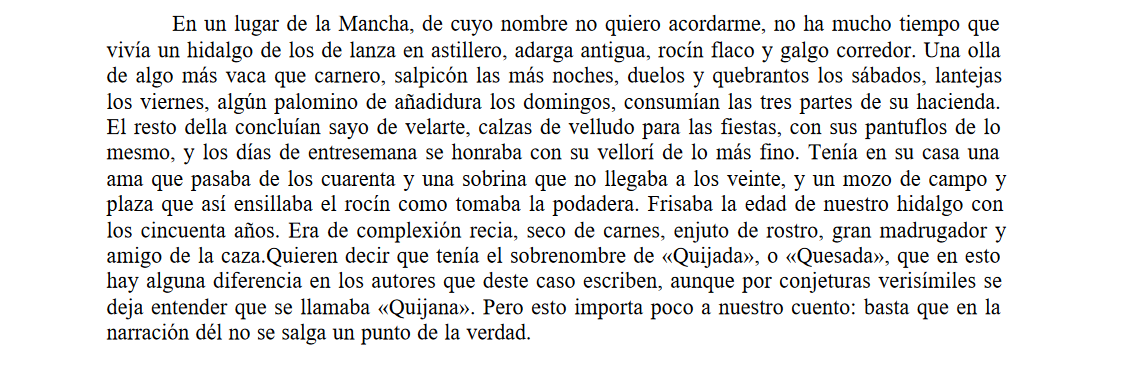
\includegraphics[width=1.10\textwidth]{Imagenes/Ejemplos/Cap1DonQuijote}
	\caption{Texto original de Don Quijote de la Mancha}
	\label{fig:Quijote}
\end{figure} 


\begin{figure}[htb]
	\centering
	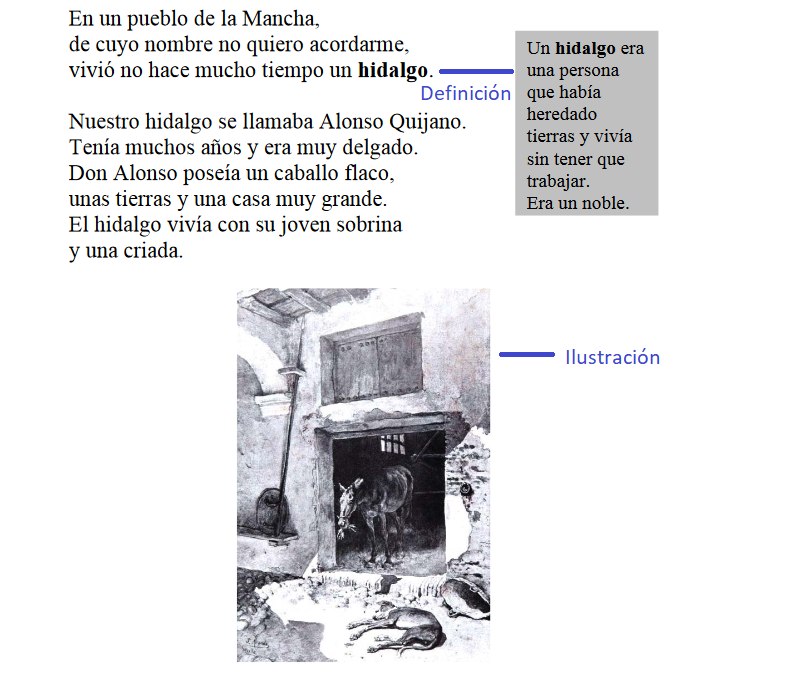
\includegraphics[width=0.8\textwidth]{Imagenes/Ejemplos/Cap1DonQuijoteLF}
	\caption{Texto LF de Don Quijote de la Mancha}
	\label{fig:QuijoteLF}
\end{figure}




\subsection{Un poco de historia}
El movimiento de la Lectura Fácil surgió en Suecia en 1968\footnote{https://www.lecturafacilextremadura.es/historia/}. En ese año se publicó el primer libro en Lectura Fácil y desde entonces hasta 1994 se crearon 330 obras, unas 15 y 20 nuevas cada año. Este movimiento se extendió a los países vecinos, Noruega y Finlandia.

 \setlength{\parskip}{10pt}
 
En Noruega, por ejemplo, la iniciativa (proyecto) se denomina \textit{Leser s$\emptyset$ker bok”}\footnote{https://lesersokerbok.no/english/} (Lector busca libro) que es una alianza de 20 organizaciones que incluyen editoriales y organizaciones de personas con discapacidad.

 \setlength{\parskip}{10pt}
 
En 1988, en Bruselas, se crea la organización \textit{Inclusion Europe \footnote{http://www.inclusion-europe.eu/}}, la alianza europea de organizaciones que trabajan por los derechos de las personas con discapacidad, en la que se agrupa a organizaciones y asociaciones de personas con discapacidad intelectual de 40 países europeos e Israel.

 \setlength{\parskip}{10pt}

En 1998, se elabora la guía \textit{«El camino más fácil: Directrices europeas para generar información de fácil lectura destinada a personas con discapacidad intelectual»\footnote{\href{http://www.lecturafacil.net/media/resources/ILSMHcastell\%C3\%A0.pdf}{http://www.lecturafacil.net/media/resources/ILSMHcastell\%C3\%A0.pdf}}} y se diseña un logotipo europeo de Lectura Fácil, para identificar todos los textos adaptados que siguen sus pautas.

 \setlength{\parskip}{10pt}
 
En 2003, en España se crea la primera Asociación de Lectura Fácil en Barcelona\footnote{https://www.lecturafacil.net/es/}. Desde entonces, surgen diversas organizaciones e iniciativas a favor de la Lectura Fácil por toda España, donde hay más de 300 libros adaptados para aquellas personas con problemas de lectura.


\subsection{Destinatarios de la Lectura Fácil} \label{subsec:gruposLectores}
La Lectura Fácil se dirige a una serie de grupos con ciertas dificultades de compresión lectora. Algunos de ellos son los siguientes: 
 
\begin{itemize}
	\item Personas con dificultades en el aprendizaje (como la dislexia, etc.)	 
	\item Personas con poca cultura o escasa escolarización.	 
	\item Personas extranjeras o inmigrantes que no dominan bien la lengua española.
	\item Niños que necesitan un refuerzo en la lectura.
	\item Personas sordas con dificultades en la comprensión.
	\item Personas mayores con trastornos mentales.
	\item Personas con hiperactividad y  déficit de atención. 
	\item Personas con discapacidad intelectual o del desarrollo (como el autismo, afasia, etc.). 
\end{itemize}
	A modo representativo de todos los colectivos que necesitan de la LF se muestra la Figura \ref{fig:destinatarios}. Los círculos representan a los grupos beneficiarios de LF, y el cuadrado la necesidad de la misma \citep{nomura2010guidelines}. 
	\begin{figure}[htb]
		\centering
		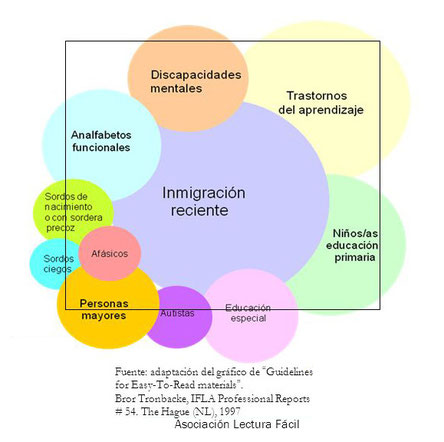
\includegraphics[width=0.8\textwidth]{Imagenes/Ejemplos/destinatarios}
		\caption{Beneficiarios de la Lectura Fácil}
		\label{fig:destinatarios}
	\end{figure}
	

	



\subsection{¿Cómo se identifican los textos de Lectura Fácil?}
Los textos adaptados a Lectura Fácil vienen identificados por dos tipos de logotipos. En la Figura \ref{fig:IFLA} podemos ver el logo que la Asociación de Lectura Fácil otorga a los textos que se adaptan a las normas de la Federación Internacional de Asociaciones de Bibliotecarios y Bibliotecas (IFLA), del inglés \textit{International Federation of Library Associations and Institutions}\footnote{\href{https://www.ifla.org/ES}{https://www.ifla.org/ES}}. Por otro lado, la Figura  \ref{fig:logoEuropeo} muestra el logo utilizado por Inclusion Europe.
\begin{figure}[htb]
\centering
	
\includegraphics[width=0.5\textwidth]{Imagenes/Logos/indice}
	\caption{Logo de Lectura Fácil que cumplen las normas de la IFLA}
	\label{fig:IFLA}
\end{figure} 
\begin{figure}[htb]
	\centering
	
\includegraphics[width=0.3\textwidth]{Imagenes/Logos/indice2}
	\caption{Logotipo europeo de Lectura Fácil}
	\label{fig:logoEuropeo}
\end{figure} 

\subsection{Pautas a seguir para la elaboración de Lectura Fácil}
Para hacer posibles las adaptaciones a LF de cualquier texto, se deben seguir una serie de directrices. Uno de los primeros documentos sobre como elaborar texto adaptado a Lectura Fácil fue publicado por la IFLA. Hay otro que fue elaborado por varias organizaciones de Inclusion Europe bajo el título ``Información para todos'' \citep{InformacionParaTodos}.


Algunas de las siguientes categorías clasificadas por Plena Inclusión \citep{LFMetodos} son:
	\begin{itemize}
\item Ortografía:
\begin{itemize}
\item Evitar el uso de algunos signos de ortografía que dificulten la comprensión del texto.
	\begin{itemize}
\item	Evitar mayúsculas excepto cuando toca según las reglas ortográficas.
	
\item	Evitar signos de ortografía poco habituales (\%, \&, /, …).
\item Usar guión para los diálogos.
\item Evitar los números romanos.
	\item Limitar el uso de la coma.


 \end{itemize}
 \end{itemize}

\item Gramática
\begin{itemize}
\item Evitar estructuras complejas que puedan dificultar la comprensión.
\begin{itemize}
	\item Usar voz activa, evitando siempre la voz pasiva y subjuntivo.
		\item No usar tiempos verbales complejos.
			\item Usar frases cortas. Escribir una idea por frase, es decir, separar cada idea por un punto o con una ``y'' en vez de una coma. 
				\item Estructurar el texto de forma clara y coherente.
 \end{itemize}
 \end{itemize}

\item Léxico:
\begin{itemize}
	\item Usar un lenguaje sencillo y directo. 
		\item Evitar la jerga y los términos técnicos. 
			\item Evitar abreviaturas.    	
 \end{itemize}

\item Estilo:

\begin{itemize}
	\item Usar la personalización, es decir, escribir de forma directa y personal. 

	\item Usar una palabra por concepto.
	

	\item Incluir imágenes relacionadas con el texto.
 \end{itemize}
 \end{itemize}
	%\item Uso de frases simples, cortas y con una estructura habitual.
	% \item Uso de imágenes sencillas y pictogramas de apoyo al texto, de manera descriptiva.
	%\item Cada frase debe ocupar una línea. Si no es fuese posible deberá ocupar varias líneas.
	% \item Evitar oraciones impersonales y pasivas reflejas.
	%\item Evitar el subjuntivo o la voz pasiva.
	%\item Evitar signos ortográficos poco habituales. (\%, \&, /, ...)
	% \item Evitar abreviaturas, acrónimos y siglas
	%\item Uso de palabras de uso cotidiano y evitar tecnicismos.
	%\item Ideas principales
	%\item Redactar en modo directo
	%\item No dar conocimientos previos por conocidos.
	%\item Evitar diseños cargados.
	%\item Eliminar información no necesaria.


\subsection{Niveles de adaptación a Lectura Fácil}
La Lectura Fácil no dispone de un estándar fijo, sino que se proponen distintos niveles ya que es imposible adaptar un texto de la misma manera para todas las personas con estas dificultades. Dicha adaptación se refiere tanto a texto como a imágenes o cualquier otro elemento que se incorpore.

La IFLA establece tres niveles, semejantes
tanto para obras originales en LF como para las adaptadas a LF:
\begin{itemize}
	\item Primer nivel: es el más sencillo y simple con muchas imágenes y escaso texto, con una dificultas sintáctica baja.
	\item Segundo nivel: es intermedio, menos sencillo que el anterior con un vocabulario y expresiones que son conocidas por todos, fácil de seguir y comprender. En este nivel también se usan imágenes.
	\item Tercer nivel: es el más complejo, con textos más extensos, con palabras poco corrientes, con saltos en el tiempo y espacio. En este nivel hay pocas imágenes.
\end{itemize}

Esta clasificación se hace en base al usuario que se dirija.



\subsection{Tareas para la simplificación de Texto}\label{subsec:tareas}

Muchas características de los textos se pueden modificar o transformar para hacerlo más legible y comprensible. El objetivo de las adaptaciones a Lectura Fácil es transformar oraciones complejas en otras más simples \citep{HoracioSaggion}. 




Los métodos de simplificación deberían facilitar o agilizar la adaptación del texto disponible, haciendo posible el acceso de la información a personas con discapacidad cognitiva. Por lo general, los textos adaptados tendrían pérdida de información y un estilo más simple,aunque no necesariamente. Podemos valorar esto positivamente, siempre y cuando el resultado final pueda ser entendido por el lector objetivo. 


Hay muchas características de los textos que pueden ser modificadas para hacerlo más legible y comprensible, incluyendo también el modo en el que se muestra. La simplificación del texto se suele basar en las siguientes cuatro tareas:  


La simplificación léxica tiene como objetivo reemplazar palabras difíciles con expresiones más fáciles de leer (o comprender) mientras se conserva el significado de los segmentos del texto original.



 \begin{itemize}
	
	\item Simplificación léxica: tiene como objetivo reemplazar las palabras difíciles por otras más fáciles (sinónimos) que se consideren mejores para comprender o leer, siempre y cuando el significado no quede alterado. Por ejemplo, ``El automóvil es de color azul'' por ``El coche es de color azul''.
	
	\item Simplificación sintáctica: tiene como objetivo transformar frases u oraciones largas que contienen figuras sintácticas que hacen ilegible e incomprensibles, transformarlas en otras más simples y en forma activa (se debe evitar siempre que se pueda la forma pasiva), en definitiva que sean legibles y comprensibles. Por ejemplo, ``China se va de fiesta, que se esta recuperando del coronavirus'' por ``China se va de fiesta. China se esta recuperando del coronavirus''. 
	
	\item Eliminar información: el objetivo es la reducción de frases u oraciones, manteniendo la información esencial, eliminando los detalles innecesarios, que no añaden nada nuevo a la idea que se quiere transmitir. Por ejemplo, ``Laura sacó a pasear a su perro, un San Bernardo, por el parque'' por ``Laura sacó a pasear a su perro por el parque''. 
	
	\item Añadir información: el objetivo es aportar conocimiento extra que pueda ayudar al lector a comprender y aprender el significado de uno o varios términos que desconozca. Por ejemplo, ``Mi vecino se compró un Ferrari'' por ``Mi vecino se compró un ferrari, un coche deportivo caro''. 
	
\end{itemize}


 Estás simplificaciones están relacionadas y en ocasiones se necesita la mezcla de ellas para mantener la coherencia y conseguir el texto final.




\section{Movimientos y asociaciones de Lectura Fácil}
Surgen en España una serie de movimientos con el fin de integrar y favorecer a las personas con dificultades en la comprensión lectora, la información y cultura a través de materiales de lectura adaptados. Algunos de ellos son los siguientes:


\begin{itemize}
	\item{\textbf{Asociación de Lectura Fácil de Barcelona}\footnote{\href{https://www.lecturafacil.net/es}{{https://www.lecturafacil.net/es}}}. Esta asociación fue creada en 2003, la primera en España del movimiento LF. Es una asociación sin ánimo de lucro que trabaja para hacer fácil el acceso la lectura, cultura e información a todas las personas, en especial a aquellas con dificultades en la lectura. 
	
	\item{\textbf{Asociación Lectura Fácil Extremadura}\footnote{\href{https://www.lecturafacilextremadura.es/}{{https://www.lecturafacilextremadura.es/}}}. Es una asociación sin ánimo de lucro que trabaja a favor de la promoción, implantación y difusión de la LF. Buscan la obetnción de la Igualdad para todos y cada uno de los ciudadanos de la comunidad.
	
	\item{\textbf{Fundación Ciudadanía (Extremadura)}\footnote{\href{https://www.fundacionciudadania.es/}{https://www.fundacionciudadania.es/}}}. Fundación sin ánimo de lucro, declarada de Utilidad Pública. Realiza aportaciones y estrategias en el ámbito de la Innovación Educativa y el Empleo, extendiendo su ámbito de actuación a todo el territorio español, poniendo énfasis en Extremadura y en su vocación europea y latinoamericana.
	
	\item{\textbf{Dilee Lectura Fácil (Extremadura)}\footnote{\href{https://odsextremadura.es/dilee-lectura-facil-extremadura/}{https://odsextremadura.es/dilee-lectura-facil-extremadura/}}}. Es una empresa española, pionera en Extremadura, que pretende implantar y consolidar la Lectura Fácil en todos los ámbitos y sectores de la vida económica, socio-política, artística-cultural, educativa, etc.
	
	\item{\textbf{Lectura Fácil Madrid}\footnote{\href{https://www.lecturafacilmadrid.com/}{https://www.lecturafacilmadrid.com/}}}. Es una asociación creada en el año 2013 que tiene como finalidad  lograr que todas las personas puedan participar de forma activa y responsable en la sociedad y hacer realidad la democracia lectora. 
	
	\item{\textbf{Cooperativa Altavoz (Madrid)}\footnote{\href{http://altavozcooperativa.org/}{http://altavozcooperativa.org/}}}. Es una cooperativa formada por personas con discapacidad
	que trabaja para mejorar la autonomía de todas las personas, adaptando contenidos a lectura fácil.
	
	\item{\textbf{Lectura Fácil Euskadi (Bilbao)}\footnote{\href{https://lecturafacileuskadi.net/}{https://lecturafacileuskadi.net/}}}.Es una asociación que pretende incentivar la creación, difusión y utilización de materiales en Lectura Fácil, a través de un programa de animación a la lectura dirigido a personas con dificultad lectora.
	
	\item{\textbf{Lectura Fácil Castilla y León (Palencia)}\footnote{\href{http://www.lecturafacyl.es/}{http://www.lecturafacyl.es/}}}. Es una entidad sin ánimo de lucro que trabaja para difundir la Lectura Fácil como herramienta de conocimiento entre las personas con dificultades de comprensión lectora en Castilla y León.
	
	\item{\textbf{Instituto de Lectura Fácil (Sevilla)}\footnote{\href{http://www.institutolecturafacil.org/}{http://www.institutolecturafacil.org/}}}. Es una organización social con el objetivo de reivindicar el derecho que tenemos a comprender la información que nos rodea, dar calidad de vida a la ciudadanía, en especial de los colectivos más vulnerables de la sociedad.
	
		\item{\textbf{Plena Inclusión}\footnote{\href{https://www.plenainclusion.org/}{https://www.plenainclusion.org/}}}. Es una organización, formada por 17 federaciones autonómicas (Ceuta y Melilla también) y unas 900 asociaciones en toda España, que representa a las personas con discapacidad intelectual o del desarrollo.	Defienden los derechos y fomentan la calidad de vida de personas con discapacidad intelectual o del desarrollo y su familia. 
		
	%\item{\textbf{diloFácil}\footnote{\href{http://www.dilofacil.es/}{http://www.dilofacil.es/}}}. Adaptan textos en Lectura Fácil para una comunicación más accesible.Han adaptado la Constitución española en Lectura Fácil
	
		\item{\textbf{SOLCOM}}\footnote{\href{https://asociacionsolcom.org/}https://asociacionsolcom.org/}}}. Organización no gubernamental, independiente y orientada a dar asistencia legal para la solidaridad comunitaria de las personas con diversidad funcional y la inclusión social.
		
\end{itemize}

\clearpage

\section{Proyectos y materiales adaptados a la Lectura Fácil}

Existen diversos proyectos que fomentan el uso de la Lectura Fácil. Han sido creados prospectos, manuales, guías, documentos y noticias para facilitar el acceso a la información a aquellos que lo necesiten. 


\subsection{Guía en Lectura Fácil sobre los servicios del banco}



Plena inclusión Galicia ha publicado una guía en LF \citep{GuiaBanco}, el 21 de julio de 2020, sobre cómo realizar operaciones básicas a través de los diferentes servicios que ofrece un banco, como crear una cuenta, controlar los movimientos, etc.

\subsection{Guía de uso del Metro de Madrid en Lectura fácil}


En esta guía adaptada a LF \citep{GuiaMetro}, tiene como objetivo contribuir a que las personas con discapacidad intelectual puedan moverse por la red del suburbano de forma autónoma. Fue publicada por Plena Inclusión en el año 2019 y ha sido revisada y actualizada en 2020. 

\subsection{Guía y plano accesible del Museo del Prado} 
Es la primera guía  de Lectura Fácil \citep{GuiaMuseo}, elaborada por el Museo del Prado con la colaboración de Plena Inclusión, ofreciendo una selección de 10 obras maestras ubicadas en el plano accesible \citep{plano} que le acompaña, para facilitar la visita de personas con discapacidad cognitiva. Ha recibido el premio CERMI.ES 2019 en la categoría de Accesibilidad Universal – Fundación Vodafone España.

\subsection{{Noticias Fácil} }
Noticias Fácil\footnote{\href{http://www.noticiasfacil.es/}{http://www.noticiasfacil.es/}} es un proyecto de Discapnet, creado en noviembre del 2013, en el marco del Plan Avanza del Ministerio de Industria, Comercio y Turismo de España. Es una plataforma interactiva de servicios y contenidos web adaptados a LF relacionados con la actualidad. Es una web de acceso libre, sin tener que ingresar ningún tipo de dato. Cuenta con 8 secciones: ¿Qué es lectura Fácil?, noticias, biblioteca, agenda, encuestas y vocabulario. Este portal está pensado para que lo pueda leer todo el mundo, en un lenguaje sencillo y claro. Además, cualquier persona puede enviar noticias, algo de actualidad o de importancia en su vida.

\subsection{Proyecto de Lectura Fácil sobre COVID-19}

Un grupo de investigadoras de la Facultad de Psicología, junto con la Universidad Católica, con la colaboración de la Clínica Universidad de los Andes, ambas ubicadas en Chile, y la casa de estudios, elaboran un documento sobre la COVID-19 en formato de LF \citep{covid}, publicado el 4 de noviembre del 2020.
El objetivo de este documento es que las personas con discapacidad cognitiva, puedan comprender de manera más fácil la nueva enfermedad que hay en la actualidad.


\section{Programas y aplicaciones de Lectura Fácil}

En está sección veremos algunas aplicaciones creadas por asociaciones, grupos y movimientos que trabajan la comprensión lectora para mejorar la lectura, practicar y aprender vocabulario.

\subsection{Dytective para dislexia }
Dytective para dixlexia \citep{rello2018superar} es una herramienta diseñada para niños que ayuda a mejorar las habilidades con o sin dificultades de lectura y escritura, mientras se divierten jugando. Posee una serie de niveles personalizados para cada niño que hace que se superen día a día, realizando 4 retos semanales. Incluye también, una prueba orientativa que detecta si tienes dificultades lecto-escritura.
Es una aplicación gratuita disponible tanto para Android como para iOs. Para su descarga podemos visitar la página web /url{https://www.changedyslexia.org/}. Última actualización el 24 de marzo del 2020. En la Figura \ref{fig:dytective} se muestra unos interfaces que se podrán encontrar en la aplicación.


\begin{figure}[h]
	\centering
	\subfloat{
		\label{f:inicio}
		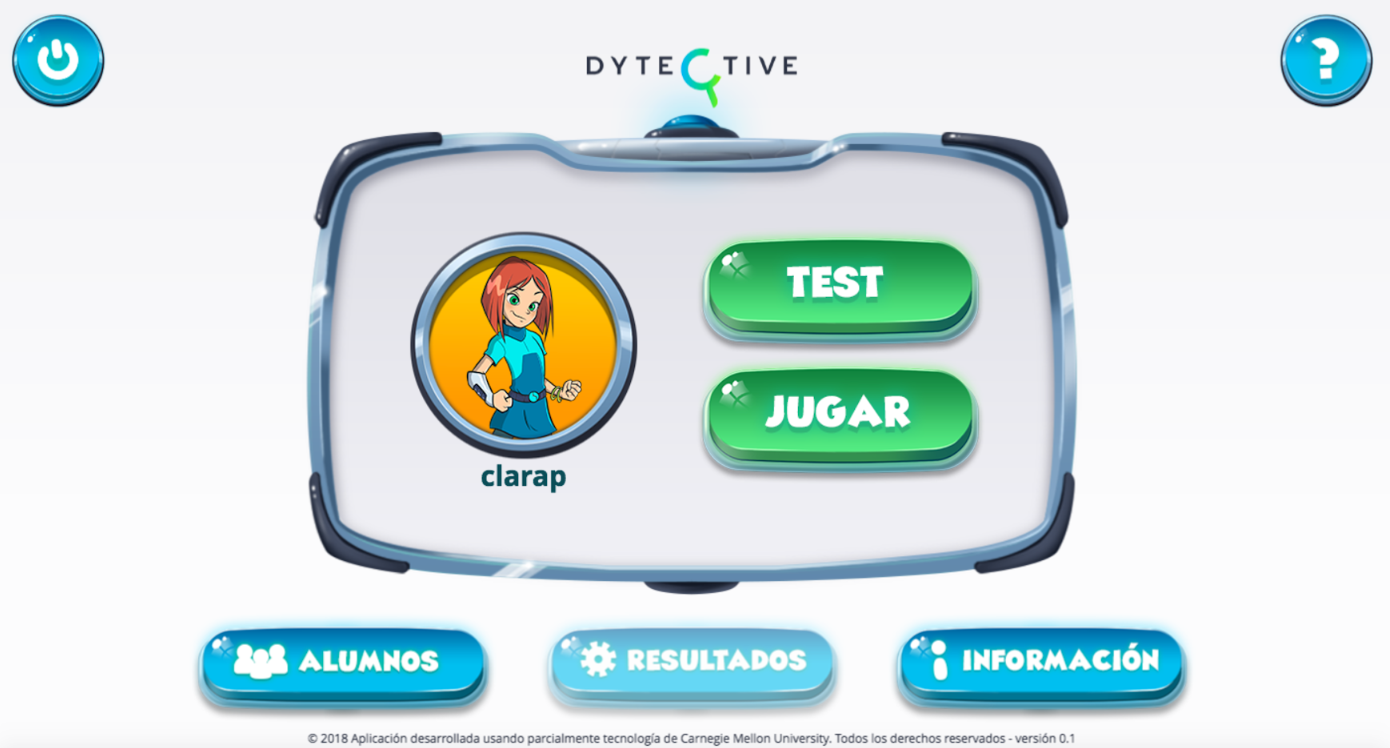
\includegraphics[width=0.5\textwidth]{Imagenes/ProyectosMateriales/dytective1}}
	\subfloat{
		\label{f:juego}
		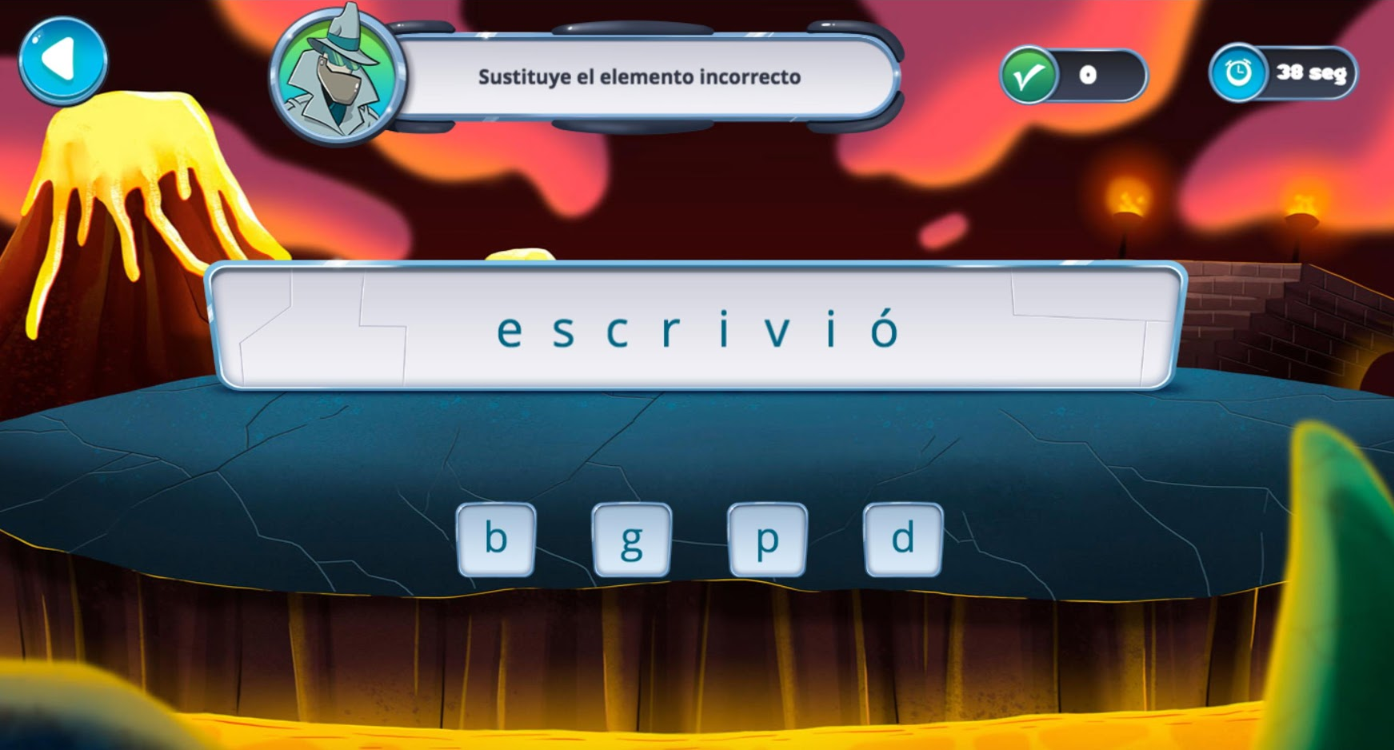
\includegraphics[width=0.5\textwidth]{Imagenes/ProyectosMateriales/dytective}}

	\caption{Aplicación Dytective para dislexia}
	\label{fig:dytective}
\end{figure}

\subsection{Léelo Fácil Educ. - Gallego }
Léelo Fácil Educ. - Gallego\footnote{\href{https://apkpure.com/es/l\%C3\%A9elo-f\%C3\%A1cil-educ-gallego/com.oneclick.ga.rayoluna}{Instalación APK ``Léelo Fácil`` en https://apkpure.com/es/l\%C3\%A9elo-f\%C3\%A1cil-educ-gallego/com.oneclick.ga.rayoluna}} es una aplicación que sirve para leer un libro adaptado a Lectura Fácil. Cuenta con dibujos, música y animaciones para un mejor entendimiento. Está aplicación es un proyecto de FEAPS Confederación (ahora Plena Inclusión) publicada el 13 de abril del 2015. La aplicación tiene dos partes: obras de relevancia para consultar a modo educativo (Dos Leyendas de Bécquer) y obras para disfrutar como ocio (Novela de Jordi Sierra i Fabra). Actualmente se encuentra disponible un APK para su descarga. Este proyecto se ha quedado obsoleto. En la Figura \ref{fig:leeloFacil} se puede ver un fragmento del libro ''El rayo de luna'' de Gustavo Adolfo Bécquer.

\begin{figure}[h]
	\centering
	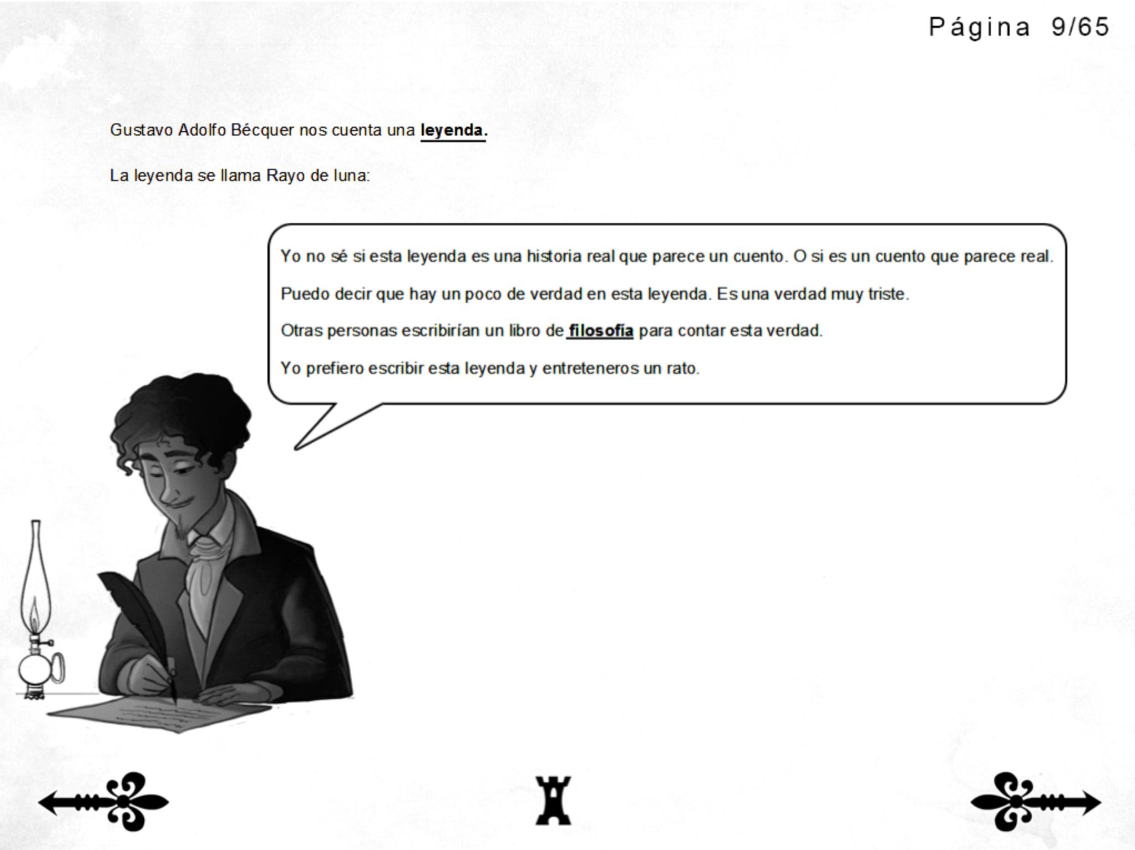
\includegraphics[width=0.9\textwidth]{Imagenes/ProyectosMateriales/leeloFacil}
	\caption{Aplicación Léelo Fácil}
	\label{fig:leeloFacil}
\end{figure} 

\subsection{Simplext }

Simplex \citep{PLN1000} es un proyecto de Able to Include financiado por el Ministerio de Industria, Turismo y Comercio, con un presupuesto de más de 2,6 millones de euros. Este proyecto es un sistema automático para la transformación de cualquier tipo de textos a LF, reduciendo la complejidad léxica y sintáctica, permitiendo así una mejor comprensión de textos. Su objetivo es el desarrollo de un producto (en este caso herramienta) que sirva de apoyo para simplificar los textos. Esta herramienta detecta las palabras y oraciones complejas, convirtiéndolas en palabras más sencillas y oraciones más cortas. Es una herramienta sencilla, se copia el texto a adaptar y se simplifica automáticamente como se muestra en la Figura \ref{fig:simplext}. En la 10ª edición de los premios BDigital a la Innovación Digital fue nominado y finalista.
Para acceder a esta herramienta podemos visitar la página web de la demo de Simplext: \url{http://simplext.taln.upf.edu/}.


\begin{figure}[h]
	\centering
	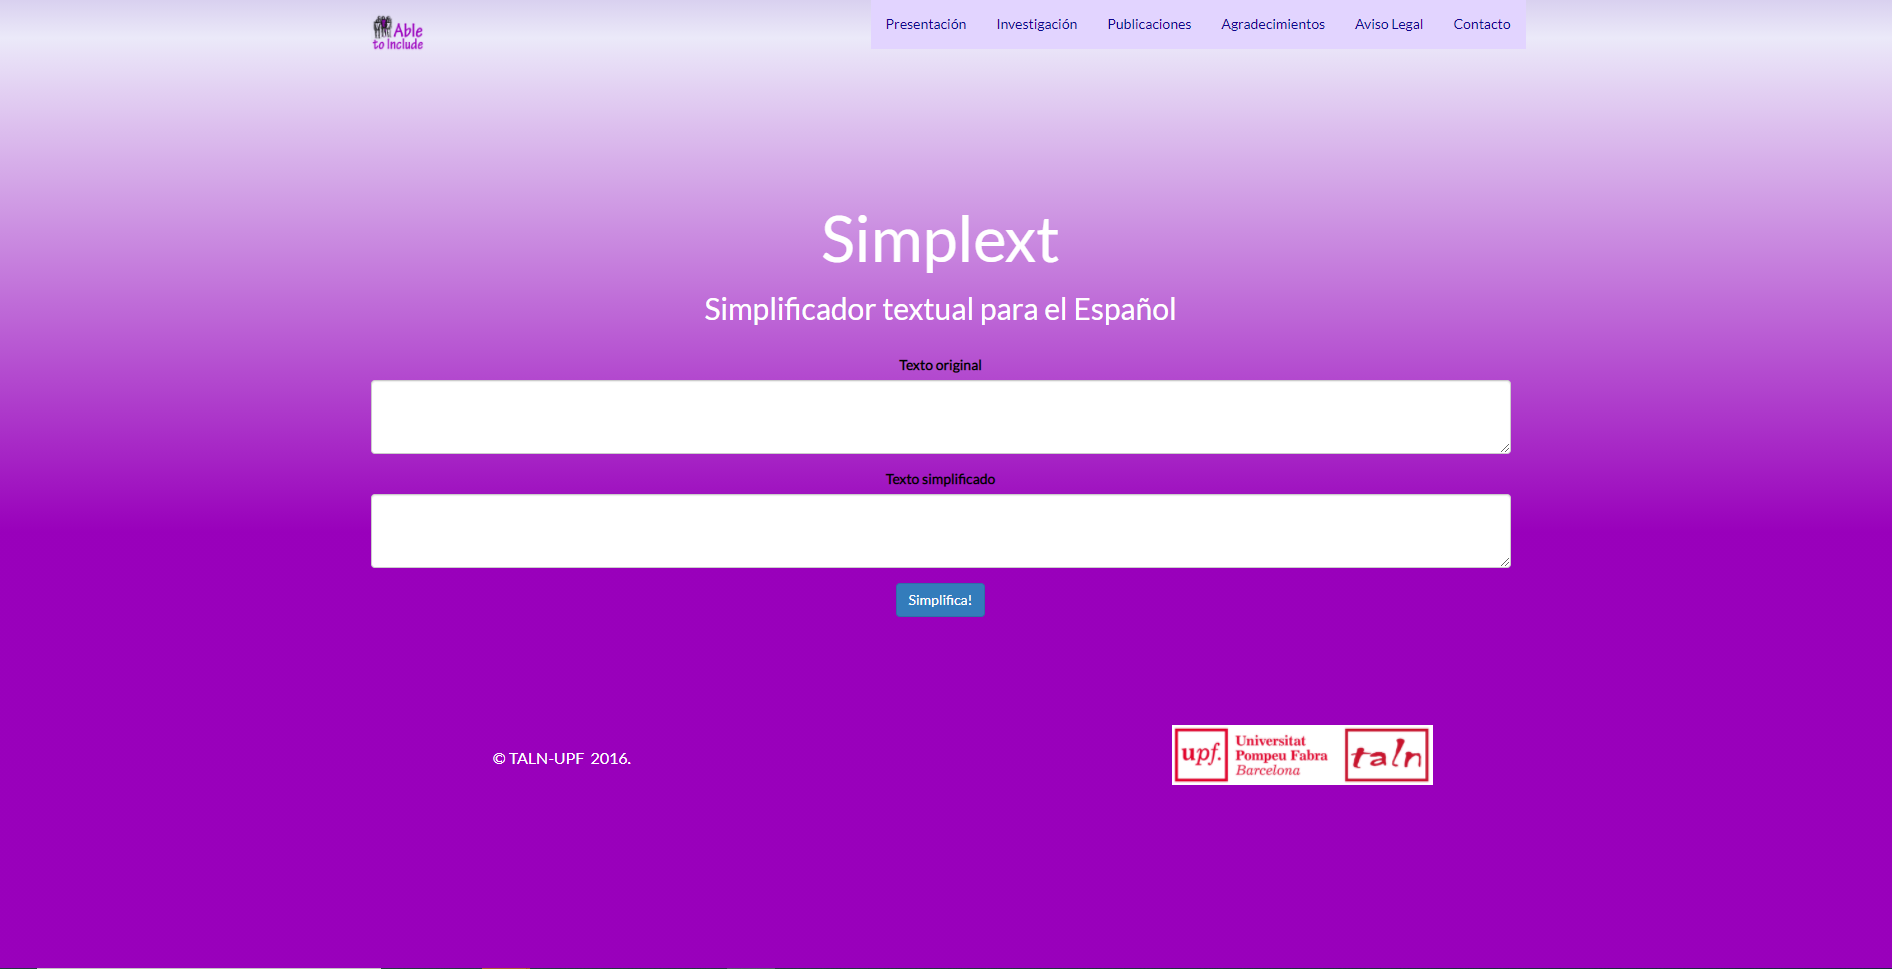
\includegraphics[width=1.0\textwidth]{Imagenes/ProyectosMateriales/simplext}
	\caption{Simplext}
	\label{fig:simplext}
\end{figure} 

\subsection{``Frente al aislamiento. Nos conectamos'' }

``Frente al aislamiento, Nos conectamos''\footnote{\href{https://my.yapp.us/ZNMC4A}{Descarga de la aplicación ``Frente al aislamiento. Nos conectamos'' en https://my.yapp.us/ZNMC4A}} es una aplicación lanzada por Plena Inclución en marzo del 2020 para dar respuesta a las necesidades de personas con discapacidad cognitiva durante la crisis del coronavirus. Se trata de una herramienta de información, participación y consulta.

Esta herramienta nos ofrece documentos, materiales, foros de consulta para preguntar dudas y agenda de actividades. Es una aplicación gratuita tanto para Android como para iOs. En la Figura \ref{fig:plenaInclusion} se puede ver a modo ilustrativo lo que nos ofrece esta aplicación.


\begin{figure}[h]
	\centering
	\subfloat{
		\label{f:menú}
		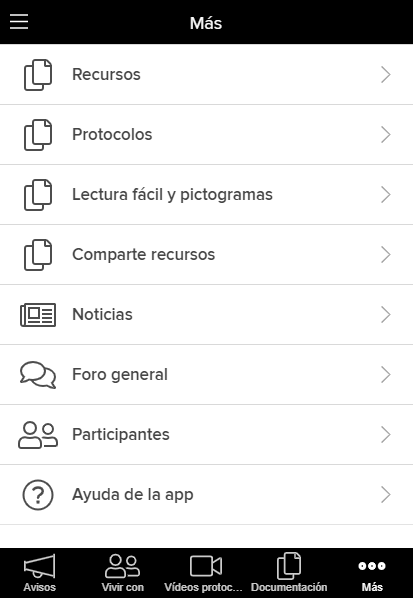
\includegraphics[width=0.5\textwidth]{Imagenes/ProyectosMateriales/plenaInclusion}}
	\subfloat{
		\label{f:avisos}
		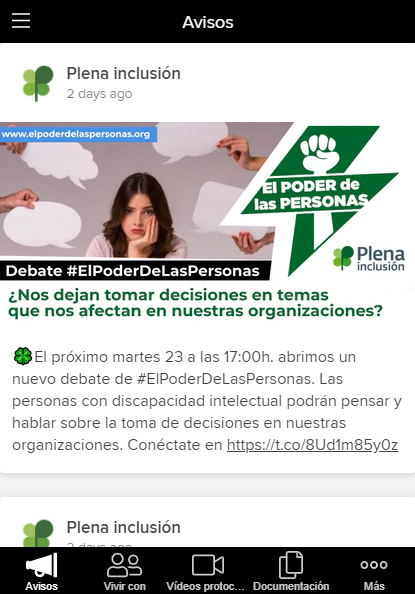
\includegraphics[width=0.5\textwidth]{Imagenes/ProyectosMateriales/plenaInclusion1}}
	
	\caption{Aplicación ``Frente al aislamiento. Nos conectamos`}
	\label{fig:plenaInclusion}
\end{figure} 


\subsection{CAPITO }

CAPITO\footnote{\href{https://www.capito.eu/en/}{https://www.capito.eu/en/}} proviene del italiano cuyo significado es ``lo entiendo'', creada por Atempo, empresa social que trabaja por la igualdad de las personas. Es aplicación tanto para móvil, tablet o PC, disponible en lengua inglesa y alemana, que podemos ver en la Figura \ref{fig:capito}. Nos ofrecen principalmente traducciones en línea a un lenguaje fácil de entender. Dispone de 3 niveles de traducción: el A1 (breve y simple), el A2 (fácilmente comprensible) y el B1 (lenguaje coloquial), siendo el A2 y el B1 especialmente adecuados para personas con dificultades de aprendizaje y discapacidades. 
También podemos encontrar cursos online para el auto-aprendizaje de escritura a LF, talleres, etc. El idioma de enseñanza es el alemán.
\begin{figure}[h]
	\centering
	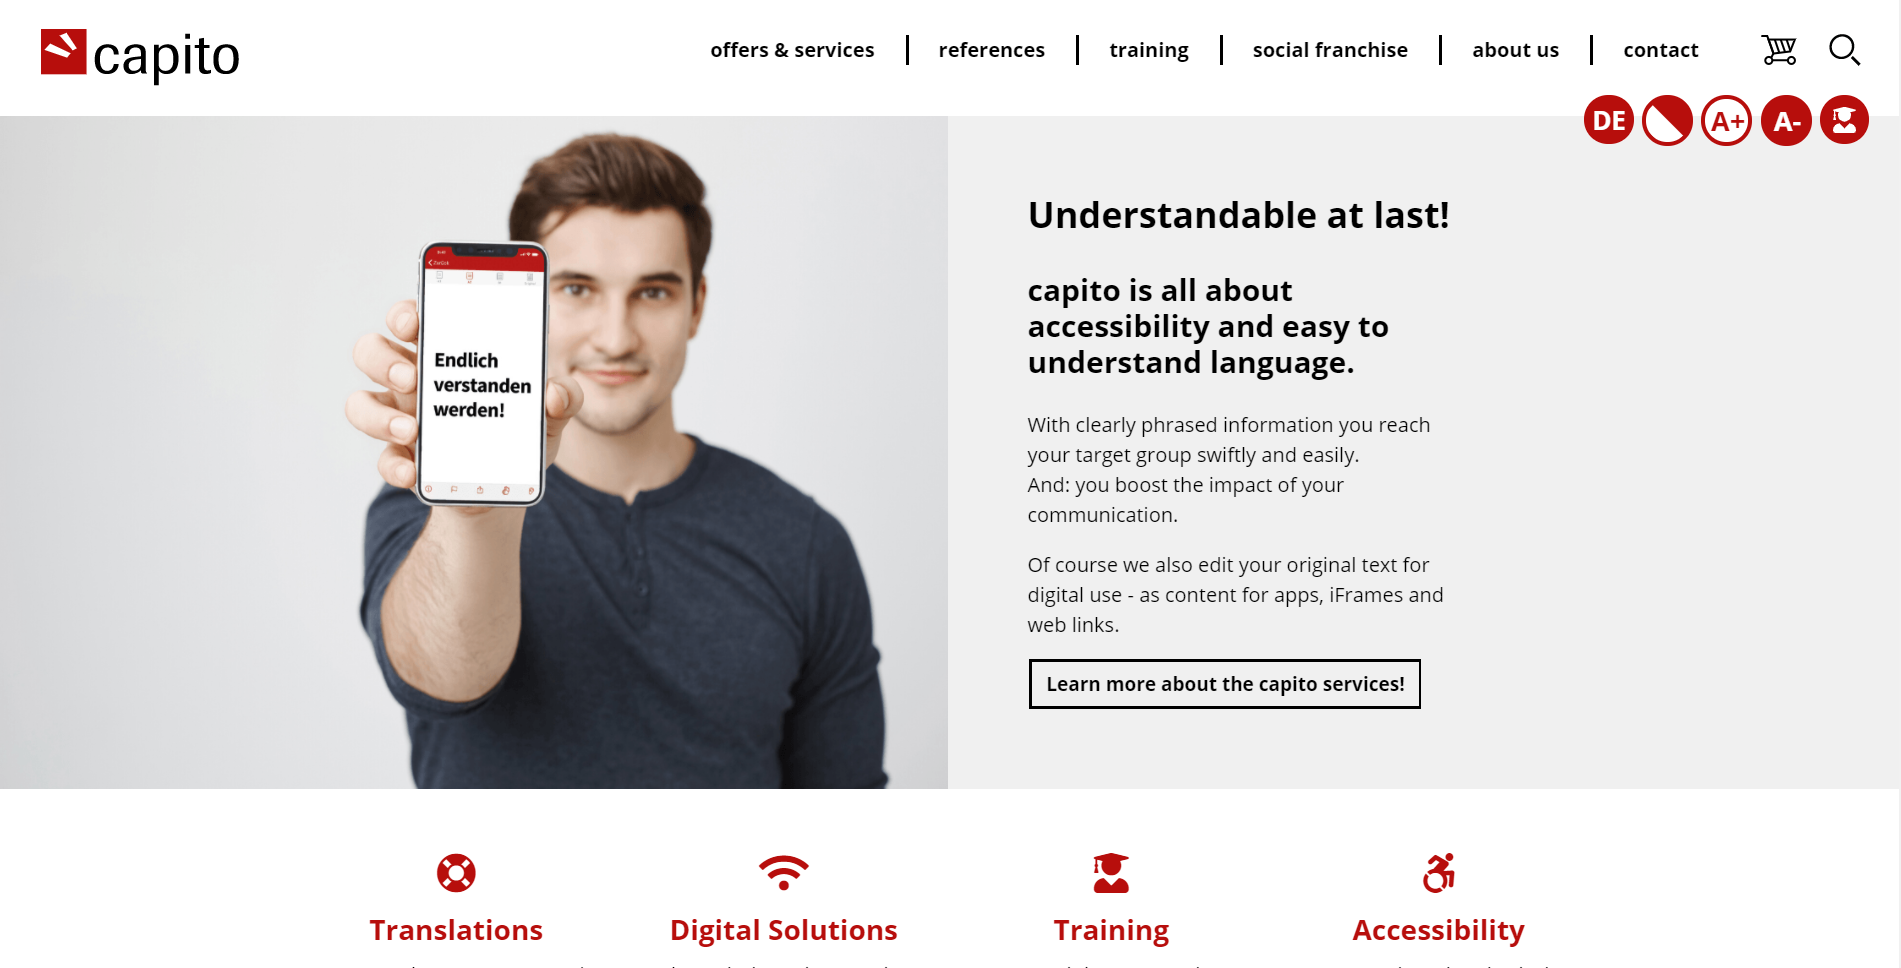
\includegraphics[width=0.8\textwidth]{Imagenes/ProyectosMateriales/capito}
	\caption{CAPITO}
	\label{fig:capito}
\end{figure} 


\subsection{SIMPATICO }

SIMPATICO\footnote{\href{https://simpatico-project.com/}{https://simpatico-project.com/}} es una plataforma cuyo objetivo es mejorar las comunicaciones e interacciones entre usuario y administración pública, a través de servicios electrónicos.
de software que recopila e integra las técnicas avanzadas desarrolladas en el proyecto SIMPATICO y las implementa sobre los sistemas de sonido 
existentes para la prestación de servicios en línea. Permite a los usuarios tener una interacción más fácil, adaptación del texto a su perfil, flujo de trabajo simplificado y personalizado y formularios web precargados con los datos personales del usuario.
Cuando algo no está claro para un determinado usuario, la simplificación del texto es a través de Text Adaptation Engine, sugiriendo cambios en el texto (léxico, sintáctico o semántico) y traducción, sinónimos y explicaciones. 

Esta plataforma también pretende fomentar la participación del usuario en la administración pública, para que puedan publicar y resolver dudas sobre trámites administrativos, entendiéndo mejor de forma visual los procesos administrativos. Este proyecto se inició el 1 de marzo del 2016 y finalizó el 28 de febrero del 2019. En la figura \ref{fig:simpatico} podemos ver el sitio web del proyecto.


\begin{figure}[h]
	\centering
	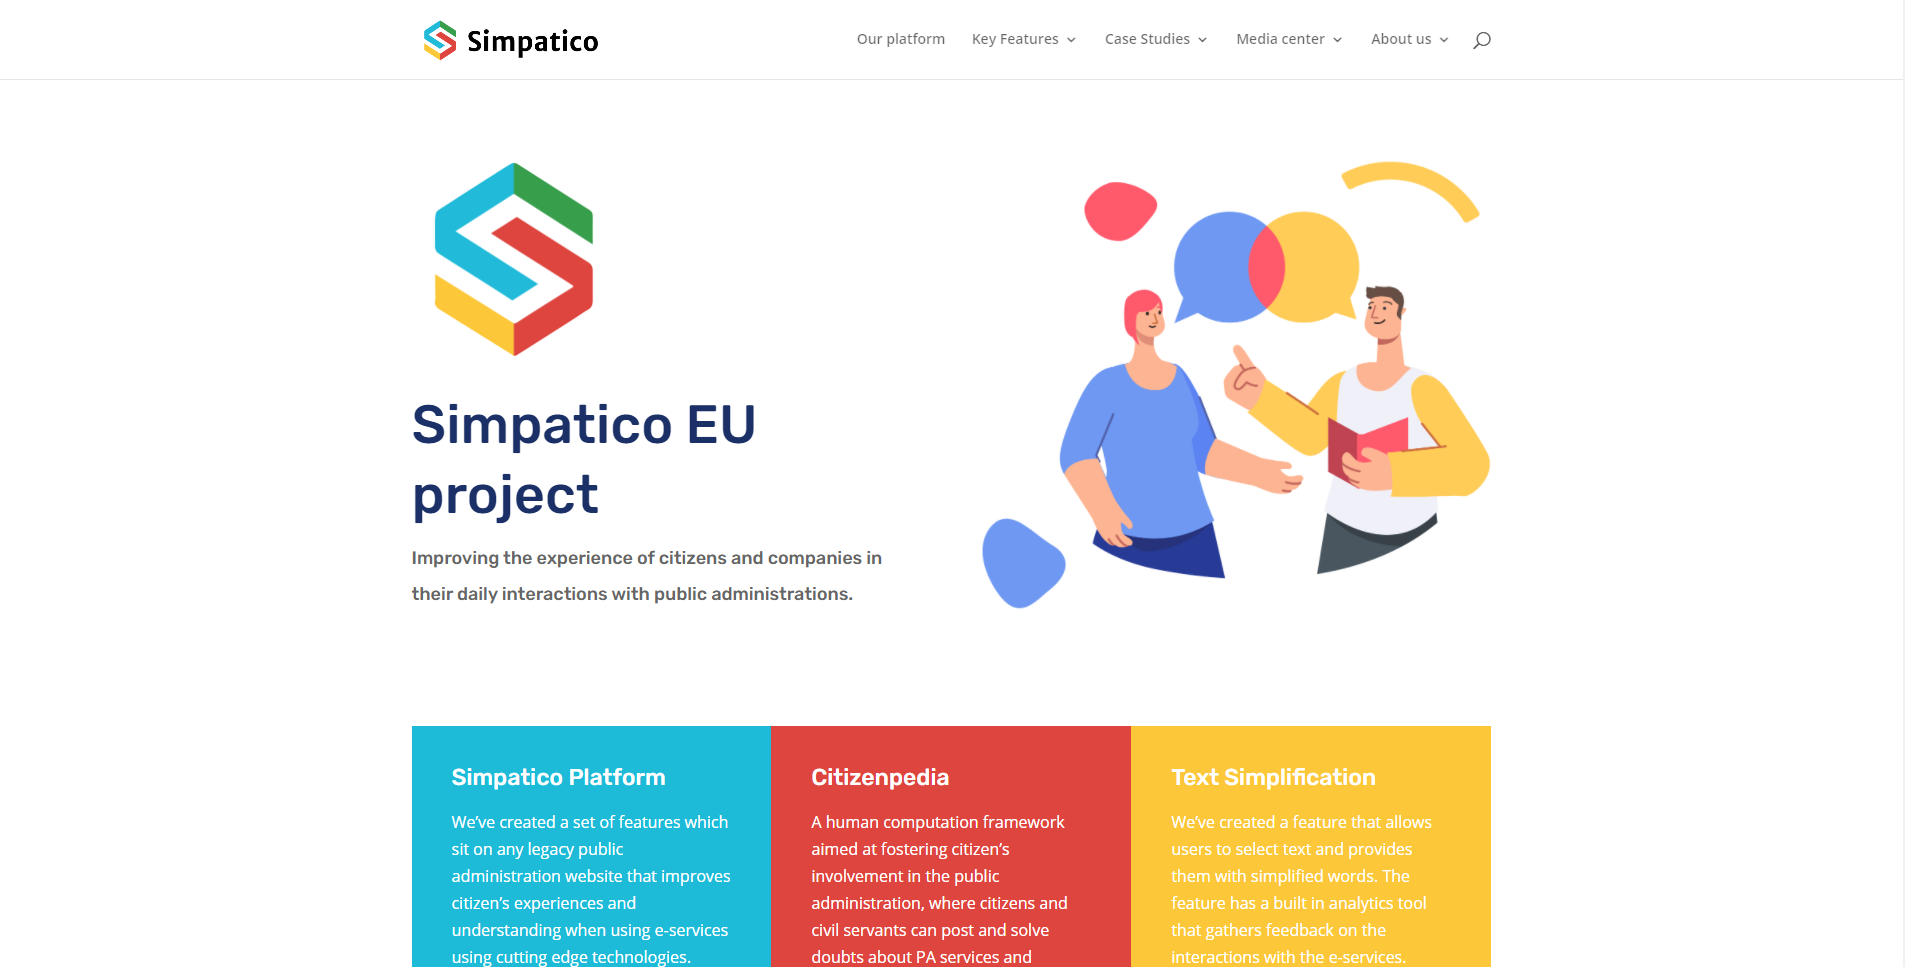
\includegraphics[width=1.0\textwidth]{Imagenes/ProyectosMateriales/simpatico}
	\caption{SIMPATICO}
	\label{fig:simpatico}
\end{figure} 




\subsection{Proyecto FIRST}

FIRST\footnote{\href{http://www.openbooktool.net/}{http://www.openbooktool.net/}} es un proyecto europeo para el desarrollo de una herramienta multilingüe, llamada Open Book \citep{openBook}, para la creación de contenidos accesibles para personas con autismo. Este proyecto empezó el 1 de octubre del 2009 y finalizó el 30 de septiembre del 2014.
El proyecto tiene como objetivo el uso de las tecnologías del lenguaje, capaces de detectar y simplificar un contenido, para que puede se más fácil de comprender, así como el impacto que tendrá de mejora en la vida de esas personas. 

A través de la herramienta online Open Book, que podemos ver en la Figura \ref{fig:openBook}, se puede simplificar textos escritos en 3 idiomas (inglés, español y búlgaro), permitiendo una personalización y adaptación a cada tipo de usuario. La conversión se hace por la detección automática de carácter lingüístico en aquello que puede dificultar la comprensión, de tal forma que el resultado final no se vea alterado respecto al contenido original. Tiene dos perfiles: modo cuidador, que ofrece más posibilidades de revisión, edición y corrección automática de texto, y modo usuario final (persona con autismo). 


\begin{figure}[h]
	\centering
	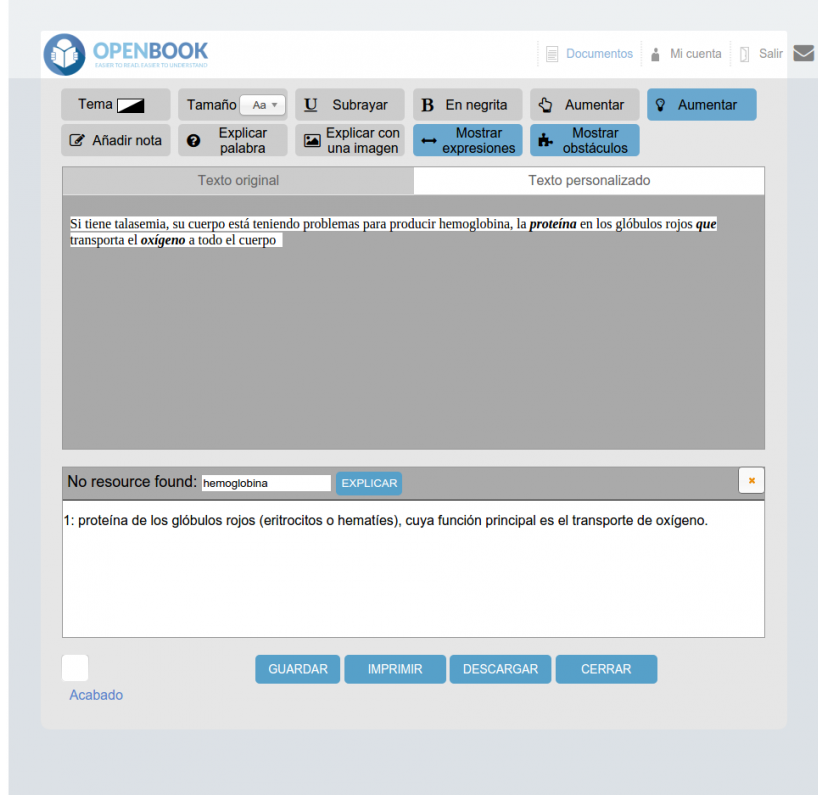
\includegraphics[width=0.6\textwidth]{Imagenes/ProyectosMateriales/openBook}
	\caption{Open Book}
	\label{fig:openBook}
\end{figure} 

\subsection{Wheris }

Wheris\footnote{\href{http://www.tematicblog.com/WHERIS\_Web//}{Se puede descargar en http://www.tematicblog.com/WHERIS\_Web/}} es una aplicación gratuita para móvil disponible tanto para iOs y android. Creada en 2016, y galardonada como mejor aplicación de nueva creación con el premio ``Best New App''. Esta aplicación detecta códigos invisibles en todos los impresos y en las reproducciones de audio y video a tu alrededor. Permite a los usuarios con discapacidad visual o dificultades de compresión lectora acceso a información que, en su versión original, no es accesible para este colectivo. En la Figura \ref{fig:wheris} se puede ver como es la aplicación.



\begin{figure}[h]
	\centering
	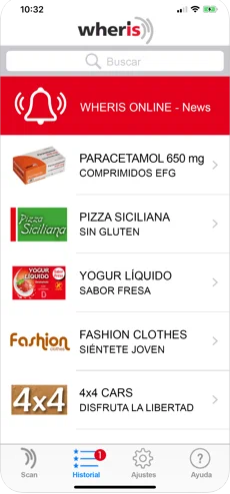
\includegraphics[width=0.5\textwidth]{Imagenes/ProyectosMateriales/wheris}
	\caption{Wheris}
	\label{fig:wheris}\end{figure} 








%En el estado de la cuestión es donde aparecen gran parte de las referencias bibliográficas del trabajo. Una de las formas más cómodas de gestionar la bibliografía en {\LaTeX} es utilizando \textbf{bibtex}. Las entradas bibliográficas deben estar en un fichero con extensión \textit{.bib} (con esta plantilla se proporcionan 3, dos de los cuales están vacíos). Cada entrada bibliográfica tiene una clave que permite referenciarla desde cualquier parte del texto con los siguiente comandos:

%\begin{itemize}
%\item Referencia bibliografica con cite: \cite{ldesc2e}
%\item Referencia bibliográfica con citep: \citep{notsoshort}
%\item Referencia bibliográfica con citet: \citet{latexAPrimer}
%\end{itemize}

%Es posible citar más de una fuente, como por ejemplo %\citep{latexCompanion,LaTeXLamport,texKnuth}

%Después, latex se ocupa de rellenar la sección de bibliografía con las entradas \textbf{que hayan sido citadas} (es decir, no con todas las entradas que hay en el .bib, sino sólo con aquellas que se hayan citado en alguna parte del texto).

%Bibtex es un programa separado de latex, pdflatex o cualquier otra cosa que se use para compilar los .tex, de manera que para que se rellene correctamente la sección de bibliografía es necesario compilar primero el trabajo (a veces es necesario compilarlo dos veces), compilar después con bibtex, y volver a compilar otra vez el trabajo (de nuevo, puede ser necesario compilarlo dos veces). 
